

\begin{figure*}[h]
	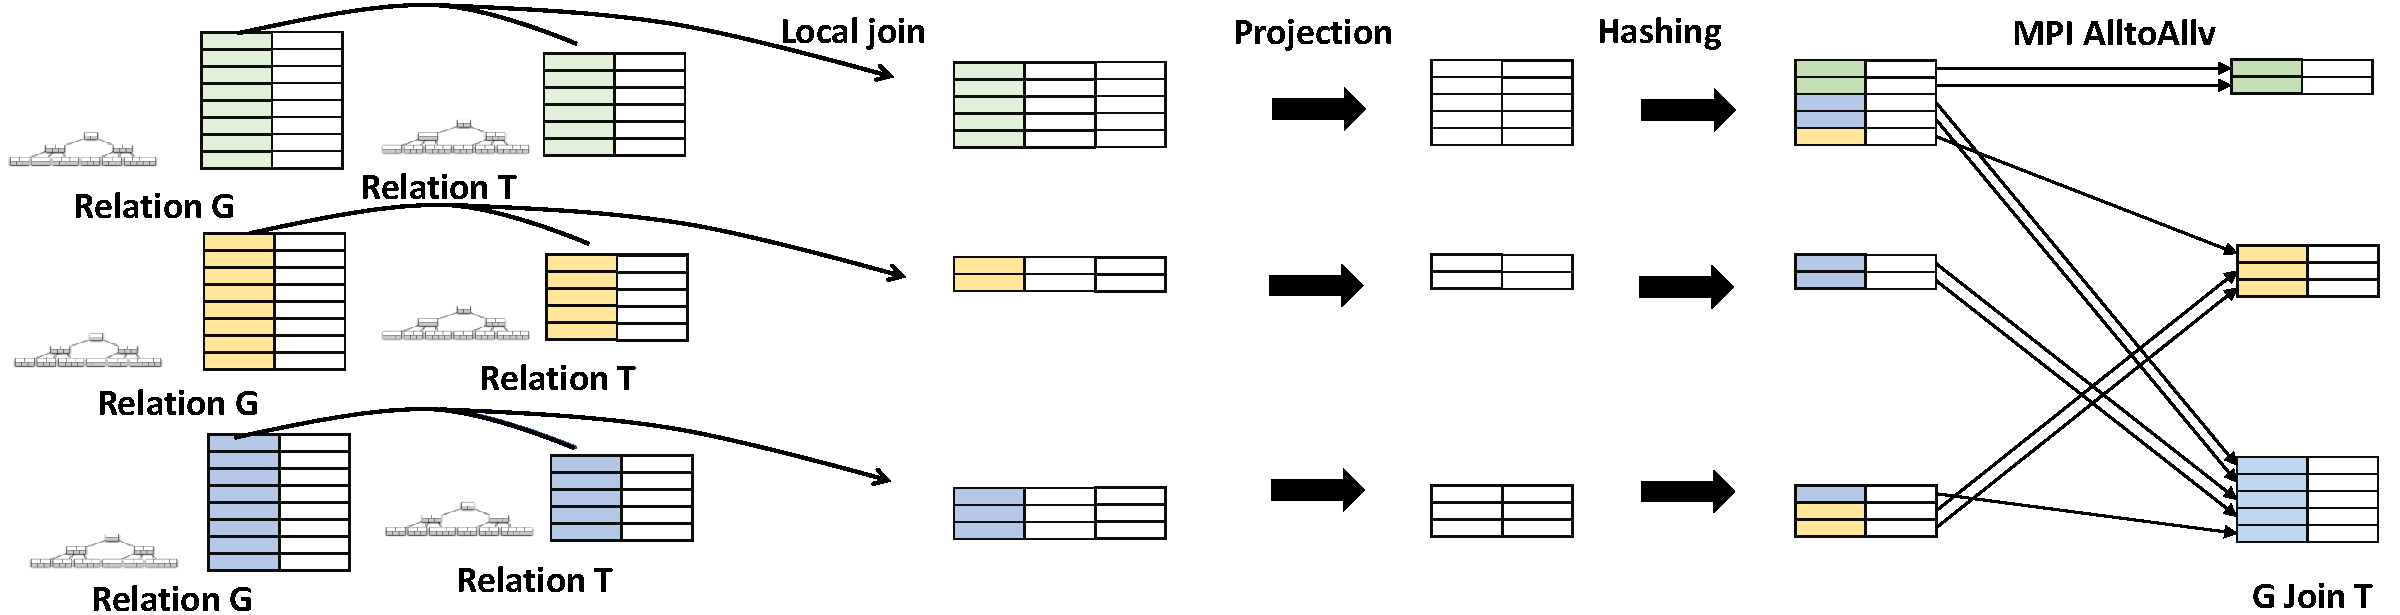
\includegraphics[width=\textwidth]{results/join_new.pdf}
	\caption{Schematic Diagram to show different phases of hash-tree join.}
	\label{fig:join}
\end{figure*}



\section{Hash-Tree Relational Algebra}
\label{sec:impl}
%
This section discusses our implementation of distributed relational algebra. We employ a hybrid approach we call \emph{hash-tree} relational algebra that consists of nesting B-tree key-value stores within a hash-table that can be partitioned across multiple cores or MPI nodes. As discussed in the previous section, the key-value store approach to encoding relations requires nested maps to support efficient join (and select) operations. In a typical join, it will be necessary to iterate over all tuples in a relation where particular columns match a value or values taken from the first operand of join---in which case the variable being matched should come first and be a key in the outermost B-tree. The relation is thus explicitly indexed on this column.

In our implementation, a relation $R(a,b)$ indexed on $a$ is encapsulated in a type \texttt{Relation<Relation<void>>} which provides an interface to a B-tree mapping \texttt{uint64\_t} keys, storing each $a$, to subrelations over just those values $b$ that are paired with a particular $a$. In our approach, this nesting of B-trees is extended at the top-level by a hash table so that each value $a$ is also hashed to one of $\mathit{nproc}$ (the number of MPI processes being used to host the relation) \textit{buckets}.

\paragraph{Hybrid join} The standard way to parallelize the key-value store approach to relational algebra on multi-core systems is to partition the iteration space of the outermost loop. For example, the Souffl\`e Datalog solver uses OpenMP to parallelize its join operations, first partitioning the outermost key-value store into multiple disjoint iterators---one for each available thread. Souffl\`e's join algorithm is nearly identical to our previous pseudocode for join, except that it adds an outer parallel for loop.   

\begin{verbatim}
      new_delta_path = {}
      pfor part_iter in delta_path.partition():
         for [x,y] in part_iter:
            for [y,z] in edge.select("y", y):
               if path.insert([x,z]) == true:
                  new_delta_path.insert([x,z])
      delta_path = new_delta_path   
\end{verbatim}


\subsection{Distributed hash-tree join}

Our hybrid hash-tree structure for relations makes this partitioning explicit as physically separate relations stored in distinct hash-table buckets---each owned by a dedicated MPI process. Join operations then decompose into a separate join for each bucket, followed by hashing of output tuples, and a communication phase to insert these tuples into the output relation. In experiments designing our join operation, we found that, as hashing distributes key values evenly across buckets, MPI's all-to-all communication paradigm was actually most efficient for inserting output tuples in their receiving buckets (i.e., on processes hosting in the output relation).

In Figure~\ref{fig:join} we show the process for computing a single iteration of a distributed transitive closure computation. $T$ (i.e., $T_\Delta$ as we implement an incrementalized TC algorithm) is joined with $G$ on a per-bucket basis (the diagram shows three color-coded buckets). Tuples in $T(x,y)$ are indexed on the second column ($y$) and tuples in $G(y,z)$ are indexed on the first column ($y$). This makes it possible to perform local (intra-bucket) joins as each tuple $(x,y) \in T$ is guaranteed to have all matching tuples $(y,z) \in G$ stored in the same bucket, managed by the same MPI process. Each resulting triple $(x,y,z)$ has its middle column projected out on-the-fly as it is produced, and, as the resulting tuple $(x,z)$ must be inserted into $T$, a relation indexed on its second column, each new edge is hashed and assigned to bucket $\mathit{hash}(z)\%\mathit{nprocs}$ in the output relation ($T$). As this bucket will likely not be managed by the local MPI process, a communication phase is required to actually perform insertion of each output tuple in its output relation. As each output tuple is produced it is staged in one of $\mathit{nprocs}$ packets, ready to be sent across the network to the MPI process managing its bucket. Finally, an all-to-all communication phase is used to reorganize the output of the join operation---preparing $T$ for subsequent fixed-point iterations. As tuples are received by their host process, they are inserted into the local B-tree structure, eliminating duplicates.  


\subsection{Distributed hash-tree union}

\begin{figure*}[h]
	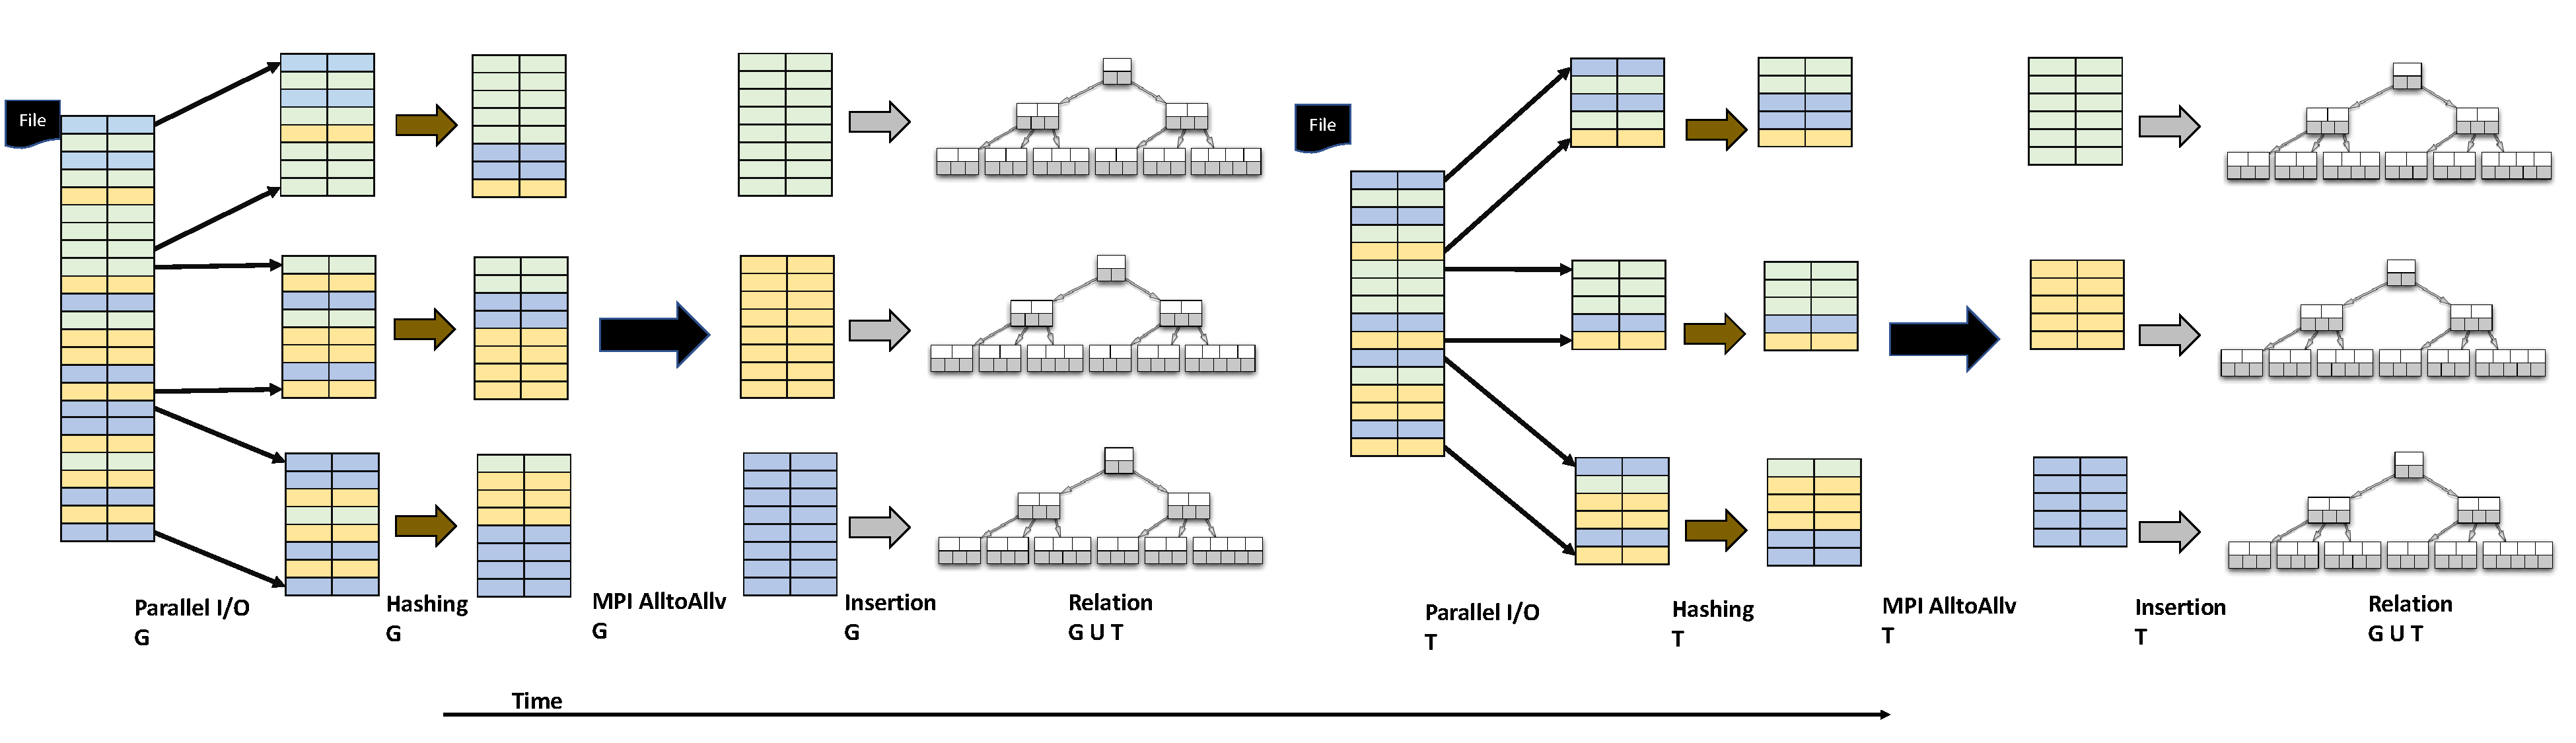
\includegraphics[width=\textwidth]{results/union_1.pdf}
	\caption{Schematic Diagram to show different phases of naive hash-tree union.}
	\label{fig:union_1}
\end{figure*}

We present two algorithms for distributed unions, na\"ive hash-tree union and buffered hash-tree union. As the name suggests buffered hash-tree union buffers data across all relations that need to be unioned before performing any communication or insertions and performs the union concurrently in a single step. While performing a union of $n$ relations, na\"ive hash-tree union involves $n$ epochs of communication and computation---one for each relation---as opposed to buffered hash-tree union (see Figure~\ref{fig:union_2}) that uses buffering to limit the number of communication and computation epochs to one.

Na\"ive hash-tree union (see Figure~\ref{fig:union_1}) is concurrent in processing each relation being unioned, but unions each relation in a separate step. Naturally, our buffered implementation has an extra memory overhead as opposed to the na\"ive implementation where all graphs that need to be unioned are processed one at a time, however it is more representative of real applications (such as Datalog, program analysis, etc) where each relation being unioned would have a set of nodes hosting it and tuples across multiple relations could all be transmitted and inserted into a new relation concurrently.

\begin{figure}[h]
	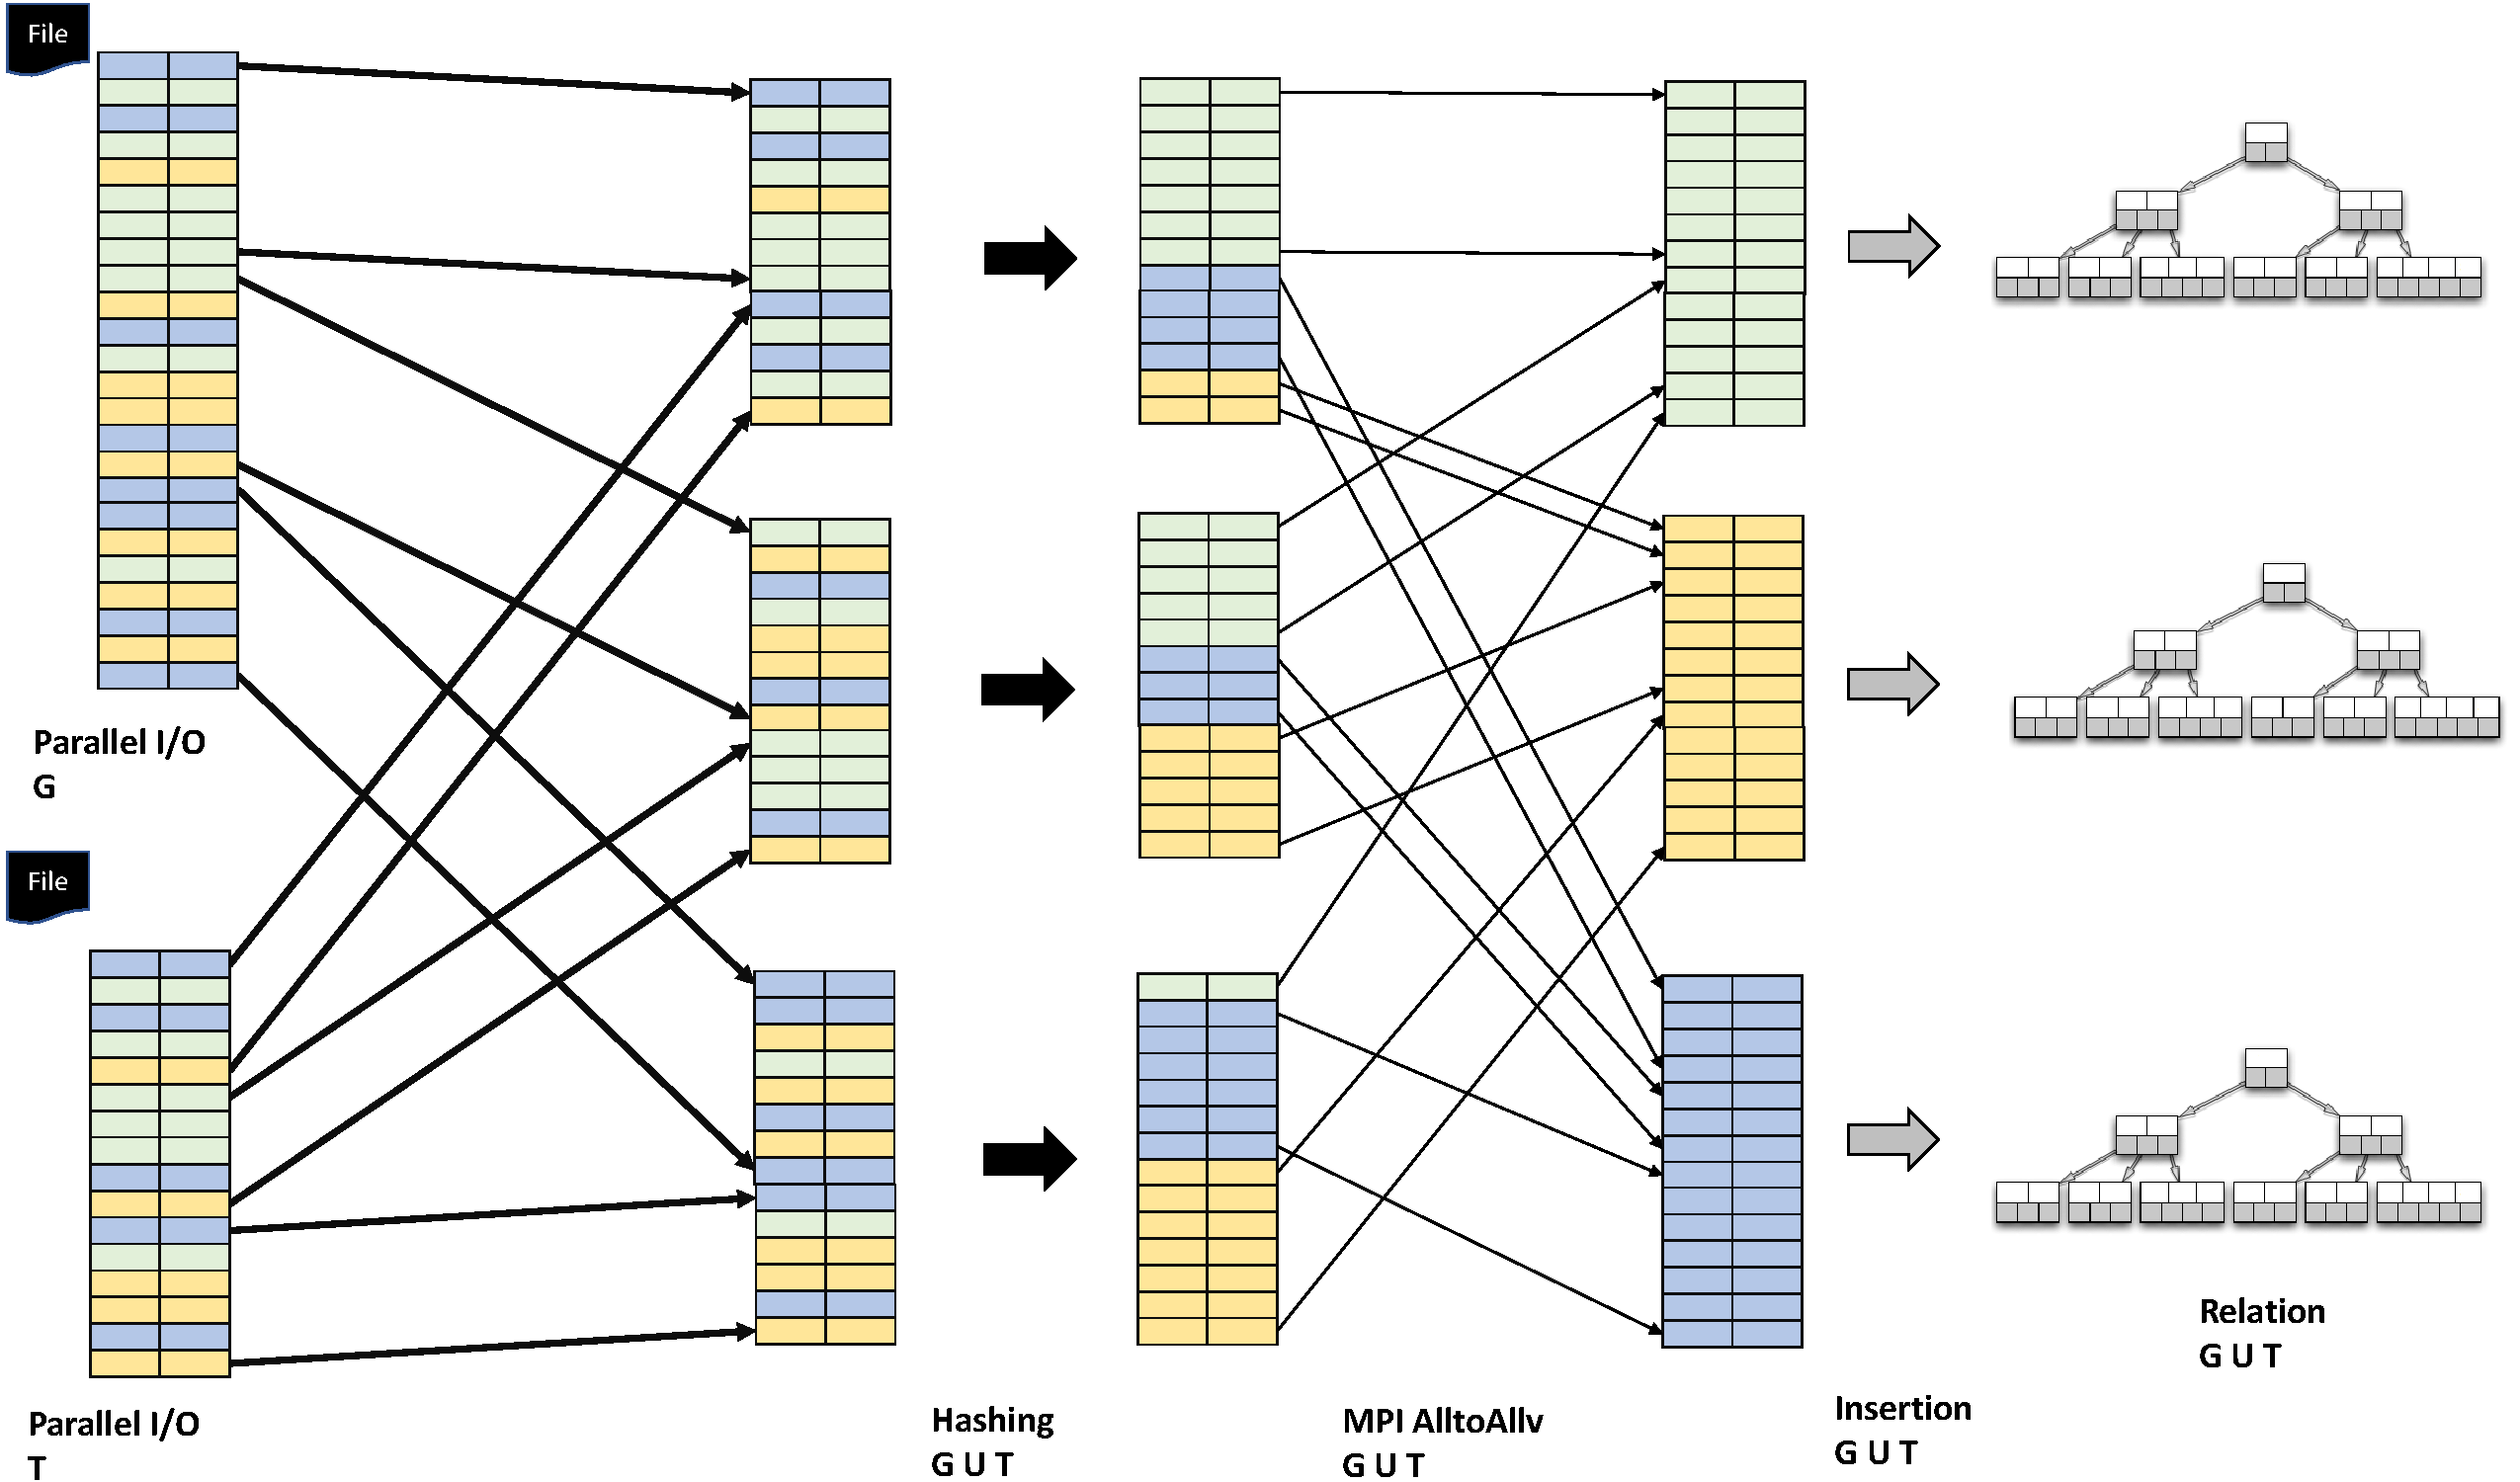
\includegraphics[width=\columnwidth]{results/union_2.pdf}
	\caption{Schematic Diagram to show different phases of buffered hash-tree union.}
	\label{fig:union_2}
\end{figure}

The input graphs can be read from files stored on the disk or can be read directly from memory. If the graphs are read from disk, the first phase is that of parallel I/O: processes access disjoint regions of the file to read an equal number of tuples in parallel. Once the tuples are read into memory, each process scans through its tuples and hashes them, grouping tuples into $\mathit{nprocs}$ packets, ready to be sent across the network. The target process (i.e., outer hash-bucket) of a tuple is computed based on the hash value of its key. For instance, the target rank of a two column tuple $(a, b)$, where $a$ is the outer key and $b$ the inner key, would be $\mathit{hash}(a)\%\mathit{nprocs}$. We also perform preliminary deduplication, as these tuples are staged, before transmitting these batches of tuples to minimize communication overhead. The grouping step is followed by an all-to-all communication phase where tuples are sent to the appropriate processes (outer hash buckets). Once tuples arrive at a process, they are inserted into the local relation container. This step performs the important task of deduplication of tuples across relations. 
